\documentclass[]{article}
\usepackage{lmodern}
\usepackage{amssymb,amsmath}
\usepackage{ifxetex,ifluatex}
\usepackage{fixltx2e} % provides \textsubscript
\ifnum 0\ifxetex 1\fi\ifluatex 1\fi=0 % if pdftex
  \usepackage[T1]{fontenc}
  \usepackage[utf8]{inputenc}
\else % if luatex or xelatex
  \ifxetex
    \usepackage{mathspec}
  \else
    \usepackage{fontspec}
  \fi
  \defaultfontfeatures{Ligatures=TeX,Scale=MatchLowercase}
\fi
% use upquote if available, for straight quotes in verbatim environments
\IfFileExists{upquote.sty}{\usepackage{upquote}}{}
% use microtype if available
\IfFileExists{microtype.sty}{%
\usepackage{microtype}
\UseMicrotypeSet[protrusion]{basicmath} % disable protrusion for tt fonts
}{}
\usepackage[margin=1in]{geometry}
\usepackage{hyperref}
\hypersetup{unicode=true,
            pdftitle={Species\_specific\_genes},
            pdfauthor={Lauren Blake},
            pdfborder={0 0 0},
            breaklinks=true}
\urlstyle{same}  % don't use monospace font for urls
\usepackage{color}
\usepackage{fancyvrb}
\newcommand{\VerbBar}{|}
\newcommand{\VERB}{\Verb[commandchars=\\\{\}]}
\DefineVerbatimEnvironment{Highlighting}{Verbatim}{commandchars=\\\{\}}
% Add ',fontsize=\small' for more characters per line
\usepackage{framed}
\definecolor{shadecolor}{RGB}{248,248,248}
\newenvironment{Shaded}{\begin{snugshade}}{\end{snugshade}}
\newcommand{\KeywordTok}[1]{\textcolor[rgb]{0.13,0.29,0.53}{\textbf{#1}}}
\newcommand{\DataTypeTok}[1]{\textcolor[rgb]{0.13,0.29,0.53}{#1}}
\newcommand{\DecValTok}[1]{\textcolor[rgb]{0.00,0.00,0.81}{#1}}
\newcommand{\BaseNTok}[1]{\textcolor[rgb]{0.00,0.00,0.81}{#1}}
\newcommand{\FloatTok}[1]{\textcolor[rgb]{0.00,0.00,0.81}{#1}}
\newcommand{\ConstantTok}[1]{\textcolor[rgb]{0.00,0.00,0.00}{#1}}
\newcommand{\CharTok}[1]{\textcolor[rgb]{0.31,0.60,0.02}{#1}}
\newcommand{\SpecialCharTok}[1]{\textcolor[rgb]{0.00,0.00,0.00}{#1}}
\newcommand{\StringTok}[1]{\textcolor[rgb]{0.31,0.60,0.02}{#1}}
\newcommand{\VerbatimStringTok}[1]{\textcolor[rgb]{0.31,0.60,0.02}{#1}}
\newcommand{\SpecialStringTok}[1]{\textcolor[rgb]{0.31,0.60,0.02}{#1}}
\newcommand{\ImportTok}[1]{#1}
\newcommand{\CommentTok}[1]{\textcolor[rgb]{0.56,0.35,0.01}{\textit{#1}}}
\newcommand{\DocumentationTok}[1]{\textcolor[rgb]{0.56,0.35,0.01}{\textbf{\textit{#1}}}}
\newcommand{\AnnotationTok}[1]{\textcolor[rgb]{0.56,0.35,0.01}{\textbf{\textit{#1}}}}
\newcommand{\CommentVarTok}[1]{\textcolor[rgb]{0.56,0.35,0.01}{\textbf{\textit{#1}}}}
\newcommand{\OtherTok}[1]{\textcolor[rgb]{0.56,0.35,0.01}{#1}}
\newcommand{\FunctionTok}[1]{\textcolor[rgb]{0.00,0.00,0.00}{#1}}
\newcommand{\VariableTok}[1]{\textcolor[rgb]{0.00,0.00,0.00}{#1}}
\newcommand{\ControlFlowTok}[1]{\textcolor[rgb]{0.13,0.29,0.53}{\textbf{#1}}}
\newcommand{\OperatorTok}[1]{\textcolor[rgb]{0.81,0.36,0.00}{\textbf{#1}}}
\newcommand{\BuiltInTok}[1]{#1}
\newcommand{\ExtensionTok}[1]{#1}
\newcommand{\PreprocessorTok}[1]{\textcolor[rgb]{0.56,0.35,0.01}{\textit{#1}}}
\newcommand{\AttributeTok}[1]{\textcolor[rgb]{0.77,0.63,0.00}{#1}}
\newcommand{\RegionMarkerTok}[1]{#1}
\newcommand{\InformationTok}[1]{\textcolor[rgb]{0.56,0.35,0.01}{\textbf{\textit{#1}}}}
\newcommand{\WarningTok}[1]{\textcolor[rgb]{0.56,0.35,0.01}{\textbf{\textit{#1}}}}
\newcommand{\AlertTok}[1]{\textcolor[rgb]{0.94,0.16,0.16}{#1}}
\newcommand{\ErrorTok}[1]{\textcolor[rgb]{0.64,0.00,0.00}{\textbf{#1}}}
\newcommand{\NormalTok}[1]{#1}
\usepackage{graphicx,grffile}
\makeatletter
\def\maxwidth{\ifdim\Gin@nat@width>\linewidth\linewidth\else\Gin@nat@width\fi}
\def\maxheight{\ifdim\Gin@nat@height>\textheight\textheight\else\Gin@nat@height\fi}
\makeatother
% Scale images if necessary, so that they will not overflow the page
% margins by default, and it is still possible to overwrite the defaults
% using explicit options in \includegraphics[width, height, ...]{}
\setkeys{Gin}{width=\maxwidth,height=\maxheight,keepaspectratio}
\IfFileExists{parskip.sty}{%
\usepackage{parskip}
}{% else
\setlength{\parindent}{0pt}
\setlength{\parskip}{6pt plus 2pt minus 1pt}
}
\setlength{\emergencystretch}{3em}  % prevent overfull lines
\providecommand{\tightlist}{%
  \setlength{\itemsep}{0pt}\setlength{\parskip}{0pt}}
\setcounter{secnumdepth}{0}
% Redefines (sub)paragraphs to behave more like sections
\ifx\paragraph\undefined\else
\let\oldparagraph\paragraph
\renewcommand{\paragraph}[1]{\oldparagraph{#1}\mbox{}}
\fi
\ifx\subparagraph\undefined\else
\let\oldsubparagraph\subparagraph
\renewcommand{\subparagraph}[1]{\oldsubparagraph{#1}\mbox{}}
\fi

%%% Use protect on footnotes to avoid problems with footnotes in titles
\let\rmarkdownfootnote\footnote%
\def\footnote{\protect\rmarkdownfootnote}

%%% Change title format to be more compact
\usepackage{titling}

% Create subtitle command for use in maketitle
\newcommand{\subtitle}[1]{
  \posttitle{
    \begin{center}\large#1\end{center}
    }
}

\setlength{\droptitle}{-2em}
  \title{Species\_specific\_genes}
  \pretitle{\vspace{\droptitle}\centering\huge}
  \posttitle{\par}
  \author{Lauren Blake}
  \preauthor{\centering\large\emph}
  \postauthor{\par}
  \predate{\centering\large\emph}
  \postdate{\par}
  \date{January 17, 2018}


\begin{document}
\maketitle

The goal of this script is to explore the categories of genes enriched
in the different groups from Cormotif.

\subsection{Load in data}\label{load-in-data}

\begin{Shaded}
\begin{Highlighting}[]
\KeywordTok{library}\NormalTok{(}\StringTok{"ggplot2"}\NormalTok{)}
\KeywordTok{library}\NormalTok{(}\StringTok{"qvalue"}\NormalTok{)}
\KeywordTok{library}\NormalTok{(}\StringTok{"RColorBrewer"}\NormalTok{)}
\KeywordTok{library}\NormalTok{(}\StringTok{"topGO"}\NormalTok{)}
\end{Highlighting}
\end{Shaded}

\begin{verbatim}
Loading required package: BiocGenerics
\end{verbatim}

\begin{verbatim}
Loading required package: parallel
\end{verbatim}

\begin{verbatim}

Attaching package: 'BiocGenerics'
\end{verbatim}

\begin{verbatim}
The following objects are masked from 'package:parallel':

    clusterApply, clusterApplyLB, clusterCall, clusterEvalQ,
    clusterExport, clusterMap, parApply, parCapply, parLapply,
    parLapplyLB, parRapply, parSapply, parSapplyLB
\end{verbatim}

\begin{verbatim}
The following objects are masked from 'package:stats':

    IQR, mad, sd, var, xtabs
\end{verbatim}

\begin{verbatim}
The following objects are masked from 'package:base':

    anyDuplicated, append, as.data.frame, cbind, colMeans,
    colnames, colSums, do.call, duplicated, eval, evalq, Filter,
    Find, get, grep, grepl, intersect, is.unsorted, lapply,
    lengths, Map, mapply, match, mget, order, paste, pmax,
    pmax.int, pmin, pmin.int, Position, rank, rbind, Reduce,
    rowMeans, rownames, rowSums, sapply, setdiff, sort, table,
    tapply, union, unique, unsplit, which, which.max, which.min
\end{verbatim}

\begin{verbatim}
Loading required package: graph
\end{verbatim}

\begin{verbatim}
Loading required package: Biobase
\end{verbatim}

\begin{verbatim}
Welcome to Bioconductor

    Vignettes contain introductory material; view with
    'browseVignettes()'. To cite Bioconductor, see
    'citation("Biobase")', and for packages 'citation("pkgname")'.
\end{verbatim}

\begin{verbatim}
Loading required package: GO.db
\end{verbatim}

\begin{verbatim}
Loading required package: AnnotationDbi
\end{verbatim}

\begin{verbatim}
Loading required package: stats4
\end{verbatim}

\begin{verbatim}
Loading required package: IRanges
\end{verbatim}

\begin{verbatim}
Loading required package: S4Vectors
\end{verbatim}

\begin{verbatim}

Attaching package: 'S4Vectors'
\end{verbatim}

\begin{verbatim}
The following object is masked from 'package:base':

    expand.grid
\end{verbatim}

\begin{verbatim}
\end{verbatim}

\begin{verbatim}
Loading required package: SparseM
\end{verbatim}

\begin{verbatim}

Attaching package: 'SparseM'
\end{verbatim}

\begin{verbatim}
The following object is masked from 'package:base':

    backsolve
\end{verbatim}

\begin{verbatim}

groupGOTerms:   GOBPTerm, GOMFTerm, GOCCTerm environments built.
\end{verbatim}

\begin{verbatim}

Attaching package: 'topGO'
\end{verbatim}

\begin{verbatim}
The following object is masked from 'package:IRanges':

    members
\end{verbatim}

\begin{Shaded}
\begin{Highlighting}[]
\CommentTok{#library("biomaRt")}
\KeywordTok{library}\NormalTok{(}\StringTok{"clusterProfiler"}\NormalTok{)}
\end{Highlighting}
\end{Shaded}

\begin{verbatim}
Loading required package: DOSE
\end{verbatim}

\begin{verbatim}
DOSE v3.4.0  For help: https://guangchuangyu.github.io/DOSE

If you use DOSE in published research, please cite:
Guangchuang Yu, Li-Gen Wang, Guang-Rong Yan, Qing-Yu He. DOSE: an R/Bioconductor package for Disease Ontology Semantic and Enrichment analysis. Bioinformatics 2015, 31(4):608-609
\end{verbatim}

\begin{verbatim}
clusterProfiler v3.6.0  For help: https://guangchuangyu.github.io/clusterProfiler

If you use clusterProfiler in published research, please cite:
Guangchuang Yu., Li-Gen Wang, Yanyan Han, Qing-Yu He. clusterProfiler: an R package for comparing biological themes among gene clusters. OMICS: A Journal of Integrative Biology. 2012, 16(5):284-287.
\end{verbatim}

\begin{Shaded}
\begin{Highlighting}[]
\KeywordTok{library}\NormalTok{(}\StringTok{"org.Hs.eg.db"}\NormalTok{)}
\end{Highlighting}
\end{Shaded}

\begin{verbatim}
\end{verbatim}

\begin{Shaded}
\begin{Highlighting}[]
\KeywordTok{library}\NormalTok{(tidyverse)}
\end{Highlighting}
\end{Shaded}

\begin{verbatim}
-- Attaching packages ---------------------------------- tidyverse 1.2.1 --
\end{verbatim}

\begin{verbatim}
√ tibble  1.4.2     √ purrr   0.2.4
√ tidyr   0.7.2     √ dplyr   0.5.0
√ readr   1.1.1     √ stringr 1.3.0
√ tibble  1.4.2     √ forcats 0.2.0
\end{verbatim}

\begin{verbatim}
-- Conflicts ------------------------------------- tidyverse_conflicts() --
x stringr::boundary()      masks graph::boundary()
x dplyr::collapse()        masks IRanges::collapse()
x dplyr::combine()         masks Biobase::combine(), BiocGenerics::combine()
x dplyr::desc()            masks IRanges::desc()
x tidyr::expand()          masks S4Vectors::expand()
x dplyr::filter()          masks stats::filter()
x dplyr::first()           masks S4Vectors::first()
x dplyr::lag()             masks stats::lag()
x BiocGenerics::Position() masks ggplot2::Position(), base::Position()
x purrr::reduce()          masks IRanges::reduce()
x dplyr::regroup()         masks IRanges::regroup()
x dplyr::rename()          masks S4Vectors::rename()
x dplyr::select()          masks AnnotationDbi::select()
x purrr::simplify()        masks clusterProfiler::simplify()
x dplyr::slice()           masks IRanges::slice()
\end{verbatim}

\begin{Shaded}
\begin{Highlighting}[]
\KeywordTok{library}\NormalTok{(data.table)}
\end{Highlighting}
\end{Shaded}

\begin{verbatim}
-------------------------------------------------------------------------
\end{verbatim}

\begin{verbatim}
data.table + dplyr code now lives in dtplyr.
Please library(dtplyr)!
\end{verbatim}

\begin{verbatim}
-------------------------------------------------------------------------
\end{verbatim}

\begin{verbatim}

Attaching package: 'data.table'
\end{verbatim}

\begin{verbatim}
The following objects are masked from 'package:dplyr':

    between, first, last
\end{verbatim}

\begin{verbatim}
The following object is masked from 'package:purrr':

    transpose
\end{verbatim}

\begin{verbatim}
The following object is masked from 'package:IRanges':

    shift
\end{verbatim}

\begin{verbatim}
The following objects are masked from 'package:S4Vectors':

    first, second
\end{verbatim}

\begin{Shaded}
\begin{Highlighting}[]
\KeywordTok{library}\NormalTok{(plyr)}
\end{Highlighting}
\end{Shaded}

\begin{verbatim}
-------------------------------------------------------------------------
\end{verbatim}

\begin{verbatim}
You have loaded plyr after dplyr - this is likely to cause problems.
If you need functions from both plyr and dplyr, please load plyr first, then dplyr:
library(plyr); library(dplyr)
\end{verbatim}

\begin{verbatim}
-------------------------------------------------------------------------
\end{verbatim}

\begin{verbatim}

Attaching package: 'plyr'
\end{verbatim}

\begin{verbatim}
The following objects are masked from 'package:dplyr':

    arrange, count, desc, failwith, id, mutate, rename, summarise,
    summarize
\end{verbatim}

\begin{verbatim}
The following object is masked from 'package:purrr':

    compact
\end{verbatim}

\begin{verbatim}
The following object is masked from 'package:IRanges':

    desc
\end{verbatim}

\begin{verbatim}
The following object is masked from 'package:S4Vectors':

    rename
\end{verbatim}

\begin{verbatim}
The following object is masked from 'package:graph':

    join
\end{verbatim}

\begin{Shaded}
\begin{Highlighting}[]
\KeywordTok{library}\NormalTok{(}\StringTok{"dplyr"}\NormalTok{)}

\CommentTok{# Load colors}
\NormalTok{pal <-}\StringTok{ }\KeywordTok{c}\NormalTok{(}\KeywordTok{brewer.pal}\NormalTok{(}\DecValTok{9}\NormalTok{, }\StringTok{"Set1"}\NormalTok{), }\KeywordTok{brewer.pal}\NormalTok{(}\DecValTok{8}\NormalTok{, }\StringTok{"Set2"}\NormalTok{), }\KeywordTok{brewer.pal}\NormalTok{(}\DecValTok{12}\NormalTok{, }\StringTok{"Set3"}\NormalTok{))}

\CommentTok{# Functions for plots}

\NormalTok{bjpm<-}
\KeywordTok{theme}\NormalTok{(}
  \DataTypeTok{panel.border =} \KeywordTok{element_rect}\NormalTok{(}\DataTypeTok{colour =} \StringTok{"black"}\NormalTok{, }\DataTypeTok{fill =} \OtherTok{NA}\NormalTok{, }\DataTypeTok{size =} \DecValTok{2}\NormalTok{),}
  \DataTypeTok{plot.title =} \KeywordTok{element_text}\NormalTok{(}\DataTypeTok{size =} \DecValTok{16}\NormalTok{, }\DataTypeTok{face =} \StringTok{"bold"}\NormalTok{),}
  \DataTypeTok{axis.text.y =}  \KeywordTok{element_text}\NormalTok{(}\DataTypeTok{size =} \DecValTok{14}\NormalTok{,}\DataTypeTok{face =} \StringTok{"bold"}\NormalTok{,}\DataTypeTok{color =} \StringTok{"black"}\NormalTok{),}
  \DataTypeTok{axis.text.x =}  \KeywordTok{element_text}\NormalTok{(}\DataTypeTok{size =} \DecValTok{14}\NormalTok{,}\DataTypeTok{face =} \StringTok{"bold"}\NormalTok{,}\DataTypeTok{color =} \StringTok{"black"}\NormalTok{),}
  \DataTypeTok{axis.title.y =} \KeywordTok{element_text}\NormalTok{(}\DataTypeTok{size =} \DecValTok{14}\NormalTok{,}\DataTypeTok{face =} \StringTok{"bold"}\NormalTok{),}
  \DataTypeTok{axis.title.x=}\KeywordTok{element_blank}\NormalTok{(),}
  \DataTypeTok{legend.text =} \KeywordTok{element_text}\NormalTok{(}\DataTypeTok{size =} \DecValTok{14}\NormalTok{,}\DataTypeTok{face =} \StringTok{"bold"}\NormalTok{),}
  \DataTypeTok{legend.title =} \KeywordTok{element_text}\NormalTok{(}\DataTypeTok{size =} \DecValTok{14}\NormalTok{,}\DataTypeTok{face =} \StringTok{"bold"}\NormalTok{),}
  \DataTypeTok{strip.text.x =} \KeywordTok{element_text}\NormalTok{(}\DataTypeTok{size =} \DecValTok{14}\NormalTok{,}\DataTypeTok{face =} \StringTok{"bold"}\NormalTok{),}
  \DataTypeTok{strip.text.y =} \KeywordTok{element_text}\NormalTok{(}\DataTypeTok{size =} \DecValTok{14}\NormalTok{,}\DataTypeTok{face =} \StringTok{"bold"}\NormalTok{),}
  \DataTypeTok{strip.background =} \KeywordTok{element_rect}\NormalTok{(}\DataTypeTok{colour =} \StringTok{"black"}\NormalTok{, }\DataTypeTok{size =} \DecValTok{2}\NormalTok{))}

\NormalTok{bjp<-}
\KeywordTok{theme}\NormalTok{(}
  \DataTypeTok{panel.border =} \KeywordTok{element_rect}\NormalTok{(}\DataTypeTok{colour =} \StringTok{"black"}\NormalTok{, }\DataTypeTok{fill =} \OtherTok{NA}\NormalTok{, }\DataTypeTok{size =} \DecValTok{2}\NormalTok{),}
  \DataTypeTok{plot.title =} \KeywordTok{element_text}\NormalTok{(}\DataTypeTok{size =} \DecValTok{16}\NormalTok{, }\DataTypeTok{face =} \StringTok{"bold"}\NormalTok{),}
  \DataTypeTok{axis.text.y =}  \KeywordTok{element_text}\NormalTok{(}\DataTypeTok{size =} \DecValTok{14}\NormalTok{,}\DataTypeTok{face =} \StringTok{"bold"}\NormalTok{,}\DataTypeTok{color =} \StringTok{"black"}\NormalTok{),}
  \DataTypeTok{axis.text.x =}  \KeywordTok{element_text}\NormalTok{(}\DataTypeTok{size =} \DecValTok{14}\NormalTok{,}\DataTypeTok{face =} \StringTok{"bold"}\NormalTok{,}\DataTypeTok{color =} \StringTok{"black"}\NormalTok{),}
  \DataTypeTok{axis.title.y =} \KeywordTok{element_text}\NormalTok{(}\DataTypeTok{size =} \DecValTok{14}\NormalTok{,}\DataTypeTok{face =} \StringTok{"bold"}\NormalTok{),}
  \DataTypeTok{axis.title.x =} \KeywordTok{element_text}\NormalTok{(}\DataTypeTok{size =} \DecValTok{14}\NormalTok{,}\DataTypeTok{face =} \StringTok{"bold"}\NormalTok{),}
  \DataTypeTok{legend.text =} \KeywordTok{element_text}\NormalTok{(}\DataTypeTok{size =} \DecValTok{14}\NormalTok{,}\DataTypeTok{face =} \StringTok{"bold"}\NormalTok{),}
  \DataTypeTok{legend.title =} \KeywordTok{element_text}\NormalTok{(}\DataTypeTok{size =} \DecValTok{14}\NormalTok{,}\DataTypeTok{face =} \StringTok{"bold"}\NormalTok{),}
  \DataTypeTok{strip.text.x =} \KeywordTok{element_text}\NormalTok{(}\DataTypeTok{size =} \DecValTok{14}\NormalTok{,}\DataTypeTok{face =} \StringTok{"bold"}\NormalTok{),}
  \DataTypeTok{strip.text.y =} \KeywordTok{element_text}\NormalTok{(}\DataTypeTok{size =} \DecValTok{14}\NormalTok{,}\DataTypeTok{face =} \StringTok{"bold"}\NormalTok{),}
  \DataTypeTok{strip.background =} \KeywordTok{element_rect}\NormalTok{(}\DataTypeTok{colour =} \StringTok{"black"}\NormalTok{, }\DataTypeTok{size =} \DecValTok{2}\NormalTok{))}


\CommentTok{# Load motif data}

\NormalTok{Table_Motif <-}\StringTok{ }\KeywordTok{read.csv}\NormalTok{(}\StringTok{"/Users/laurenblake/Desktop/Endoderm_TC/ashlar-trial/data/Table_Motif.csv"}\NormalTok{)}

\KeywordTok{dim}\NormalTok{(Table_Motif)}
\end{Highlighting}
\end{Shaded}

\begin{verbatim}
[1] 8004    2
\end{verbatim}

\section{Motif 4}\label{motif-4}

\begin{Shaded}
\begin{Highlighting}[]
\NormalTok{true_false <-}\StringTok{ }\NormalTok{Table_Motif[,}\DecValTok{2}\NormalTok{] }\OperatorTok{==}\StringTok{ }\DecValTok{4}
\KeywordTok{summary}\NormalTok{(true_false)}
\end{Highlighting}
\end{Shaded}

\begin{verbatim}
   Mode   FALSE    TRUE 
logical    7817     187 
\end{verbatim}

\begin{Shaded}
\begin{Highlighting}[]
\NormalTok{true_false <-}\StringTok{ }\KeywordTok{as.numeric}\NormalTok{(true_false)}

\CommentTok{# Merge ENSG with true/false}

\NormalTok{test_gene <-}\StringTok{ }\KeywordTok{as.vector}\NormalTok{(true_false)}
\KeywordTok{names}\NormalTok{(test_gene) <-}\StringTok{ }\NormalTok{Table_Motif[,}\DecValTok{1}\NormalTok{]}

\CommentTok{# Run topGO}
\NormalTok{go_data <-}\StringTok{ }\KeywordTok{new}\NormalTok{(}\StringTok{"topGOdata"}\NormalTok{,}
                   \DataTypeTok{ontology =} \StringTok{"BP"}\NormalTok{,}
                   \DataTypeTok{allGenes =}\NormalTok{ test_gene, }
                    \DataTypeTok{geneSel =} \ControlFlowTok{function}\NormalTok{(allScore)\{}
    \KeywordTok{return}\NormalTok{(allScore }\OperatorTok{>}\StringTok{ }\FloatTok{0.01}\NormalTok{)}
\NormalTok{\},}
                   \DataTypeTok{nodeSize =} \DecValTok{5}\NormalTok{,}
                   \DataTypeTok{annotationFun =}\NormalTok{ annFUN.org,}
                   \DataTypeTok{mapping =} \StringTok{"org.Hs.eg.db"}\NormalTok{,}
                   \DataTypeTok{ID =} \StringTok{"ensembl"}\NormalTok{)}
\end{Highlighting}
\end{Shaded}

\begin{verbatim}

Building most specific GOs .....
\end{verbatim}

\begin{verbatim}
    ( 8429 GO terms found. )
\end{verbatim}

\begin{verbatim}

Build GO DAG topology ..........
\end{verbatim}

\begin{verbatim}
    ( 12447 GO terms and 28743 relations. )
\end{verbatim}

\begin{verbatim}

Annotating nodes ...............
\end{verbatim}

\begin{verbatim}
    ( 7115 genes annotated to the GO terms. )
\end{verbatim}

\begin{Shaded}
\begin{Highlighting}[]
\CommentTok{# Perform enrichment test}
\NormalTok{go_test <-}\StringTok{ }\KeywordTok{runTest}\NormalTok{(go_data, }\DataTypeTok{algorithm =} \StringTok{"weight01"}\NormalTok{, }\DataTypeTok{statistic =} \StringTok{"fisher"}\NormalTok{)}
\end{Highlighting}
\end{Shaded}

\begin{verbatim}

             -- Weight01 Algorithm -- 

         the algorithm is scoring 3152 nontrivial nodes
         parameters: 
             test statistic: fisher
\end{verbatim}

\begin{verbatim}

     Level 17:  2 nodes to be scored    (0 eliminated genes)
\end{verbatim}

\begin{verbatim}

     Level 16:  9 nodes to be scored    (0 eliminated genes)
\end{verbatim}

\begin{verbatim}

     Level 15:  24 nodes to be scored   (11 eliminated genes)
\end{verbatim}

\begin{verbatim}

     Level 14:  50 nodes to be scored   (75 eliminated genes)
\end{verbatim}

\begin{verbatim}

     Level 13:  80 nodes to be scored   (299 eliminated genes)
\end{verbatim}

\begin{verbatim}

     Level 12:  123 nodes to be scored  (743 eliminated genes)
\end{verbatim}

\begin{verbatim}

     Level 11:  205 nodes to be scored  (1759 eliminated genes)
\end{verbatim}

\begin{verbatim}

     Level 10:  315 nodes to be scored  (2556 eliminated genes)
\end{verbatim}

\begin{verbatim}

     Level 9:   402 nodes to be scored  (3771 eliminated genes)
\end{verbatim}

\begin{verbatim}

     Level 8:   414 nodes to be scored  (4738 eliminated genes)
\end{verbatim}

\begin{verbatim}

     Level 7:   477 nodes to be scored  (5510 eliminated genes)
\end{verbatim}

\begin{verbatim}

     Level 6:   450 nodes to be scored  (6198 eliminated genes)
\end{verbatim}

\begin{verbatim}

     Level 5:   311 nodes to be scored  (6563 eliminated genes)
\end{verbatim}

\begin{verbatim}

     Level 4:   182 nodes to be scored  (6767 eliminated genes)
\end{verbatim}

\begin{verbatim}

     Level 3:   86 nodes to be scored   (6905 eliminated genes)
\end{verbatim}

\begin{verbatim}

     Level 2:   21 nodes to be scored   (6966 eliminated genes)
\end{verbatim}

\begin{verbatim}

     Level 1:   1 nodes to be scored    (7035 eliminated genes)
\end{verbatim}

\begin{Shaded}
\begin{Highlighting}[]
\NormalTok{go_table <-}\StringTok{ }\KeywordTok{GenTable}\NormalTok{(go_data, }\DataTypeTok{weightFisher =}\NormalTok{ go_test,}
                         \DataTypeTok{orderBy =} \StringTok{"weightFisher"}\NormalTok{, }\DataTypeTok{ranksOf =} \StringTok{"weightFisher"}\NormalTok{,}
                         \DataTypeTok{topNodes =} \KeywordTok{sum}\NormalTok{(}\KeywordTok{score}\NormalTok{(go_test) }\OperatorTok{<}\StringTok{ }\NormalTok{.}\DecValTok{01}\NormalTok{))}

\NormalTok{go_table}
\end{Highlighting}
\end{Shaded}

\begin{verbatim}
        GO.ID                                        Term Annotated
1  GO:0045773       positive regulation of axon extension        21
2  GO:0008643                      carbohydrate transport        71
3  GO:0086002 cardiac muscle cell action potential inv...        17
4  GO:0046885 regulation of hormone biosynthetic proce...         8
5  GO:0034122 negative regulation of toll-like recepto...        11
6  GO:0086091 regulation of heart rate by cardiac cond...        13
7  GO:0032720 negative regulation of tumor necrosis fa...        14
8  GO:0061298 retina vasculature development in camera...        11
9  GO:0006704         glucocorticoid biosynthetic process         5
10 GO:0019896           axonal transport of mitochondrion         5
11 GO:0071875       adrenergic receptor signaling pathway         5
12 GO:0086103 G-protein coupled receptor signaling pat...         5
13 GO:0007625                           grooming behavior         5
14 GO:0031943 regulation of glucocorticoid metabolic p...         5
15 GO:1901841 regulation of high voltage-gated calcium...         5
16 GO:0032691 negative regulation of interleukin-1 bet...         5
17 GO:0061577 calcium ion transmembrane transport via ...         5
18 GO:0045989 positive regulation of striated muscle c...         5
19 GO:0046661                    male sex differentiation        65
20 GO:0060412            ventricular septum morphogenesis        16
21 GO:0046849                             bone remodeling        29
22 GO:0007586                                   digestion        23
23 GO:0042755                             eating behavior         6
24 GO:0070933                    histone H4 deacetylation         6
25 GO:0001946                           lymphangiogenesis         6
26 GO:0007409                                axonogenesis       212
27 GO:0071108         protein K48-linked deubiquitination        19
28 GO:0048013           ephrin receptor signaling pathway        56
   Significant Expected weightFisher
1            5     0.48      9.2e-05
2            5     1.64      0.00031
3            4     0.39      0.00052
4            3     0.18      0.00062
5            3     0.25      0.00173
6            3     0.30      0.00290
7            3     0.32      0.00363
8            3     0.25      0.00499
9            2     0.12      0.00504
10           2     0.12      0.00504
11           2     0.12      0.00504
12           2     0.12      0.00504
13           2     0.12      0.00504
14           2     0.12      0.00504
15           2     0.12      0.00504
16           2     0.12      0.00504
17           2     0.12      0.00504
18           2     0.12      0.00504
19           3     1.50      0.00507
20           3     0.37      0.00540
21           4     0.67      0.00732
22           3     0.53      0.00740
23           2     0.14      0.00745
24           2     0.14      0.00745
25           2     0.14      0.00745
26          12     4.89      0.00749
27           3     0.44      0.00888
28           5     1.29      0.00907
\end{verbatim}

\begin{Shaded}
\begin{Highlighting}[]
\NormalTok{sig.genes <-}\StringTok{ }\KeywordTok{sigGenes}\NormalTok{(go_data)}

\NormalTok{goresults <-}\StringTok{ }\KeywordTok{sapply}\NormalTok{(go_table}\OperatorTok{$}\NormalTok{GO.ID, }\ControlFlowTok{function}\NormalTok{(x)}
\NormalTok{    \{}
\NormalTok{      genes<-}\KeywordTok{genesInTerm}\NormalTok{(go_data, x) }
\NormalTok{      genes[[}\DecValTok{1}\NormalTok{]][genes[[}\DecValTok{1}\NormalTok{]] }\OperatorTok\StringTok{ }\NormalTok{sig.genes]}
\NormalTok{    \})}
\end{Highlighting}
\end{Shaded}

\section{Motif 7}\label{motif-7}

\begin{Shaded}
\begin{Highlighting}[]
\NormalTok{true_false <-}\StringTok{ }\NormalTok{Table_Motif[,}\DecValTok{2}\NormalTok{] }\OperatorTok{==}\StringTok{ }\DecValTok{7}
\KeywordTok{summary}\NormalTok{(true_false)}
\end{Highlighting}
\end{Shaded}

\begin{verbatim}
   Mode   FALSE    TRUE 
logical    7318     686 
\end{verbatim}

\begin{Shaded}
\begin{Highlighting}[]
\NormalTok{true_false <-}\StringTok{ }\KeywordTok{as.numeric}\NormalTok{(true_false)}

\CommentTok{# Merge ENSG with true/false}

\NormalTok{test_gene <-}\StringTok{ }\KeywordTok{as.vector}\NormalTok{(true_false)}
\KeywordTok{names}\NormalTok{(test_gene) <-}\StringTok{ }\NormalTok{Table_Motif[,}\DecValTok{1}\NormalTok{]}

\CommentTok{# Run topGO}
\NormalTok{go_data <-}\StringTok{ }\KeywordTok{new}\NormalTok{(}\StringTok{"topGOdata"}\NormalTok{,}
                   \DataTypeTok{ontology =} \StringTok{"BP"}\NormalTok{,}
                   \DataTypeTok{allGenes =}\NormalTok{ test_gene, }
                    \DataTypeTok{geneSel =} \ControlFlowTok{function}\NormalTok{(allScore)\{}
    \KeywordTok{return}\NormalTok{(allScore }\OperatorTok{>}\StringTok{ }\FloatTok{0.01}\NormalTok{)}
\NormalTok{\},}
                   \DataTypeTok{nodeSize =} \DecValTok{5}\NormalTok{,}
                   \DataTypeTok{annotationFun =}\NormalTok{ annFUN.org,}
                   \DataTypeTok{mapping =} \StringTok{"org.Hs.eg.db"}\NormalTok{,}
                   \DataTypeTok{ID =} \StringTok{"ensembl"}\NormalTok{)}
\end{Highlighting}
\end{Shaded}

\begin{verbatim}

Building most specific GOs .....
\end{verbatim}

\begin{verbatim}
    ( 8429 GO terms found. )
\end{verbatim}

\begin{verbatim}

Build GO DAG topology ..........
\end{verbatim}

\begin{verbatim}
    ( 12447 GO terms and 28743 relations. )
\end{verbatim}

\begin{verbatim}

Annotating nodes ...............
\end{verbatim}

\begin{verbatim}
    ( 7115 genes annotated to the GO terms. )
\end{verbatim}

\begin{Shaded}
\begin{Highlighting}[]
\CommentTok{# Perform enrichment test}
\NormalTok{go_test <-}\StringTok{ }\KeywordTok{runTest}\NormalTok{(go_data, }\DataTypeTok{algorithm =} \StringTok{"weight01"}\NormalTok{, }\DataTypeTok{statistic =} \StringTok{"fisher"}\NormalTok{)}
\end{Highlighting}
\end{Shaded}

\begin{verbatim}

             -- Weight01 Algorithm -- 

         the algorithm is scoring 4828 nontrivial nodes
         parameters: 
             test statistic: fisher
\end{verbatim}

\begin{verbatim}

     Level 19:  1 nodes to be scored    (0 eliminated genes)
\end{verbatim}

\begin{verbatim}

     Level 18:  2 nodes to be scored    (0 eliminated genes)
\end{verbatim}

\begin{verbatim}

     Level 17:  4 nodes to be scored    (8 eliminated genes)
\end{verbatim}

\begin{verbatim}

     Level 16:  12 nodes to be scored   (12 eliminated genes)
\end{verbatim}

\begin{verbatim}

     Level 15:  30 nodes to be scored   (23 eliminated genes)
\end{verbatim}

\begin{verbatim}

     Level 14:  75 nodes to be scored   (103 eliminated genes)
\end{verbatim}

\begin{verbatim}

     Level 13:  138 nodes to be scored  (314 eliminated genes)
\end{verbatim}

\begin{verbatim}

     Level 12:  220 nodes to be scored  (933 eliminated genes)
\end{verbatim}

\begin{verbatim}

     Level 11:  378 nodes to be scored  (2086 eliminated genes)
\end{verbatim}

\begin{verbatim}

     Level 10:  533 nodes to be scored  (2971 eliminated genes)
\end{verbatim}

\begin{verbatim}

     Level 9:   642 nodes to be scored  (4180 eliminated genes)
\end{verbatim}

\begin{verbatim}

     Level 8:   673 nodes to be scored  (5179 eliminated genes)
\end{verbatim}

\begin{verbatim}

     Level 7:   723 nodes to be scored  (5837 eliminated genes)
\end{verbatim}

\begin{verbatim}

     Level 6:   629 nodes to be scored  (6360 eliminated genes)
\end{verbatim}

\begin{verbatim}

     Level 5:   413 nodes to be scored  (6642 eliminated genes)
\end{verbatim}

\begin{verbatim}

     Level 4:   230 nodes to be scored  (6811 eliminated genes)
\end{verbatim}

\begin{verbatim}

     Level 3:   103 nodes to be scored  (6920 eliminated genes)
\end{verbatim}

\begin{verbatim}

     Level 2:   21 nodes to be scored   (6973 eliminated genes)
\end{verbatim}

\begin{verbatim}

     Level 1:   1 nodes to be scored    (7035 eliminated genes)
\end{verbatim}

\begin{Shaded}
\begin{Highlighting}[]
\NormalTok{go_table <-}\StringTok{ }\KeywordTok{GenTable}\NormalTok{(go_data, }\DataTypeTok{weightFisher =}\NormalTok{ go_test,}
                         \DataTypeTok{orderBy =} \StringTok{"weightFisher"}\NormalTok{, }\DataTypeTok{ranksOf =} \StringTok{"weightFisher"}\NormalTok{,}
                         \DataTypeTok{topNodes =} \KeywordTok{sum}\NormalTok{(}\KeywordTok{score}\NormalTok{(go_test) }\OperatorTok{<}\StringTok{ }\NormalTok{.}\DecValTok{01}\NormalTok{))}

\NormalTok{go_table}
\end{Highlighting}
\end{Shaded}

\begin{verbatim}
        GO.ID                                        Term Annotated
1  GO:0010469             regulation of receptor activity       122
2  GO:0009611                        response to wounding       247
3  GO:0048645                      animal organ formation        22
4  GO:0045992 negative regulation of embryonic develop...        13
5  GO:2000107 negative regulation of leukocyte apoptot...        13
6  GO:0006477                           protein sulfation         5
7  GO:0048671 negative regulation of collateral sprout...         5
8  GO:0035023 regulation of Rho protein signal transdu...        70
9  GO:0070374 positive regulation of ERK1 and ERK2 cas...        55
10 GO:0008285 negative regulation of cell proliferatio...       278
11 GO:0045766         positive regulation of angiogenesis        48
12 GO:0043116 negative regulation of vascular permeabi...         6
13 GO:0050919                         negative chemotaxis        21
14 GO:0050927 positive regulation of positive chemotax...         7
15 GO:2001028 positive regulation of endothelial cell ...         7
16 GO:2000352 negative regulation of endothelial cell ...        12
17 GO:0007411                               axon guidance       114
18 GO:0055001                     muscle cell development        67
19 GO:0097094           craniofacial suture morphogenesis         8
20 GO:0001541                ovarian follicle development        24
21 GO:0050850 positive regulation of calcium-mediated ...        13
22 GO:0003151                 outflow tract morphogenesis        29
23 GO:0043433 negative regulation of DNA binding trans...        68
24 GO:0006898               receptor-mediated endocytosis       114
25 GO:0038084 vascular endothelial growth factor signa...        16
26 GO:0002087 regulation of respiratory gaseous exchan...         5
27 GO:2001214       positive regulation of vasculogenesis         5
28 GO:0060572          morphogenesis of an epithelial bud         5
29 GO:0090025           regulation of monocyte chemotaxis         5
30 GO:1902668        negative regulation of axon guidance         5
31 GO:0071363 cellular response to growth factor stimu...       294
32 GO:0001666                         response to hypoxia       174
33 GO:0003148          outflow tract septum morphogenesis        10
34 GO:0051895 negative regulation of focal adhesion as...        10
35 GO:0034121 regulation of toll-like receptor signali...        19
36 GO:0072073               kidney epithelium development        48
37 GO:0014074      response to purine-containing compound        49
38 GO:0034114 regulation of heterotypic cell-cell adhe...         6
39 GO:0010960                   magnesium ion homeostasis         6
40 GO:0036353         histone H2A-K119 monoubiquitination         6
41 GO:0009065 glutamine family amino acid catabolic pr...         6
42 GO:0031665 negative regulation of lipopolysaccharid...         6
   Significant Expected weightFisher
1           31    10.25      2.3e-08
2           37    20.76      4.3e-05
3            8     1.85      0.00018
4            6     1.09      0.00019
5            5     1.09      0.00023
6            4     0.42      0.00023
7            4     0.42      0.00023
8           19     5.88      0.00025
9           13     4.62      0.00049
10          41    23.37      0.00051
11          12     4.03      0.00051
12           4     0.50      0.00065
13           7     1.77      0.00117
14           4     0.59      0.00141
15           4     0.59      0.00141
16           5     1.01      0.00198
17          22     9.58      0.00200
18          13     5.63      0.00256
19           4     0.67      0.00263
20           7     2.02      0.00278
21           5     1.09      0.00300
22          10     2.44      0.00351
23          11     5.72      0.00407
24          20     9.58      0.00478
25           6     1.34      0.00514
26           3     0.42      0.00519
27           3     0.42      0.00519
28           3     0.42      0.00519
29           3     0.42      0.00519
30           3     0.42      0.00519
31          40    24.71      0.00567
32          19    14.62      0.00649
33           4     0.84      0.00688
34           4     0.84      0.00688
35           5     1.60      0.00702
36           7     4.03      0.00703
37          10     4.12      0.00959
38           3     0.50      0.00974
39           3     0.50      0.00974
40           3     0.50      0.00974
41           3     0.50      0.00974
42           3     0.50      0.00974
\end{verbatim}

\begin{Shaded}
\begin{Highlighting}[]
\NormalTok{sig.genes <-}\StringTok{ }\KeywordTok{sigGenes}\NormalTok{(go_data)}
\end{Highlighting}
\end{Shaded}

\section{Combine Motifs 4+7}\label{combine-motifs-47}

\begin{Shaded}
\begin{Highlighting}[]
\NormalTok{true_false <-}\StringTok{ }\NormalTok{Table_Motif[,}\DecValTok{2}\NormalTok{] }\OperatorTok{==}\StringTok{ }\DecValTok{7} \OperatorTok{|}\StringTok{ }\NormalTok{Table_Motif[,}\DecValTok{2}\NormalTok{] }\OperatorTok{==}\StringTok{ }\DecValTok{4}
\KeywordTok{summary}\NormalTok{(true_false)}
\end{Highlighting}
\end{Shaded}

\begin{verbatim}
   Mode   FALSE    TRUE 
logical    7131     873 
\end{verbatim}

\begin{Shaded}
\begin{Highlighting}[]
\NormalTok{true_false <-}\StringTok{ }\KeywordTok{as.numeric}\NormalTok{(true_false)}


\CommentTok{# Merge ENSG with true/false}

\NormalTok{test_gene <-}\StringTok{ }\KeywordTok{as.vector}\NormalTok{(true_false)}
\KeywordTok{names}\NormalTok{(test_gene) <-}\StringTok{ }\NormalTok{Table_Motif[,}\DecValTok{1}\NormalTok{]}

\CommentTok{# Run topGO}
\NormalTok{go_data <-}\StringTok{ }\KeywordTok{new}\NormalTok{(}\StringTok{"topGOdata"}\NormalTok{,}
                   \DataTypeTok{ontology =} \StringTok{"BP"}\NormalTok{,}
                   \DataTypeTok{allGenes =}\NormalTok{ test_gene, }
                    \DataTypeTok{geneSel =} \ControlFlowTok{function}\NormalTok{(allScore)\{}
    \KeywordTok{return}\NormalTok{(allScore }\OperatorTok{>}\StringTok{ }\FloatTok{0.01}\NormalTok{)}
\NormalTok{\},}
                   \DataTypeTok{nodeSize =} \DecValTok{5}\NormalTok{,}
                   \DataTypeTok{annotationFun =}\NormalTok{ annFUN.org,}
                   \DataTypeTok{mapping =} \StringTok{"org.Hs.eg.db"}\NormalTok{,}
                   \DataTypeTok{ID =} \StringTok{"ensembl"}\NormalTok{)}
\end{Highlighting}
\end{Shaded}

\begin{verbatim}

Building most specific GOs .....
\end{verbatim}

\begin{verbatim}
    ( 8429 GO terms found. )
\end{verbatim}

\begin{verbatim}

Build GO DAG topology ..........
\end{verbatim}

\begin{verbatim}
    ( 12447 GO terms and 28743 relations. )
\end{verbatim}

\begin{verbatim}

Annotating nodes ...............
\end{verbatim}

\begin{verbatim}
    ( 7115 genes annotated to the GO terms. )
\end{verbatim}

\begin{Shaded}
\begin{Highlighting}[]
\CommentTok{# Perform enrichment test}
\NormalTok{go_test <-}\StringTok{ }\KeywordTok{runTest}\NormalTok{(go_data, }\DataTypeTok{algorithm =} \StringTok{"weight01"}\NormalTok{, }\DataTypeTok{statistic =} \StringTok{"fisher"}\NormalTok{)}
\end{Highlighting}
\end{Shaded}

\begin{verbatim}

             -- Weight01 Algorithm -- 

         the algorithm is scoring 5182 nontrivial nodes
         parameters: 
             test statistic: fisher
\end{verbatim}

\begin{verbatim}

     Level 19:  1 nodes to be scored    (0 eliminated genes)
\end{verbatim}

\begin{verbatim}

     Level 18:  2 nodes to be scored    (0 eliminated genes)
\end{verbatim}

\begin{verbatim}

     Level 17:  6 nodes to be scored    (8 eliminated genes)
\end{verbatim}

\begin{verbatim}

     Level 16:  17 nodes to be scored   (12 eliminated genes)
\end{verbatim}

\begin{verbatim}

     Level 15:  40 nodes to be scored   (33 eliminated genes)
\end{verbatim}

\begin{verbatim}

     Level 14:  91 nodes to be scored   (147 eliminated genes)
\end{verbatim}

\begin{verbatim}

     Level 13:  153 nodes to be scored  (424 eliminated genes)
\end{verbatim}

\begin{verbatim}

     Level 12:  243 nodes to be scored  (1000 eliminated genes)
\end{verbatim}

\begin{verbatim}

     Level 11:  418 nodes to be scored  (2127 eliminated genes)
\end{verbatim}

\begin{verbatim}

     Level 10:  587 nodes to be scored  (3039 eliminated genes)
\end{verbatim}

\begin{verbatim}

     Level 9:   684 nodes to be scored  (4220 eliminated genes)
\end{verbatim}

\begin{verbatim}

     Level 8:   720 nodes to be scored  (5197 eliminated genes)
\end{verbatim}

\begin{verbatim}

     Level 7:   764 nodes to be scored  (5854 eliminated genes)
\end{verbatim}

\begin{verbatim}

     Level 6:   662 nodes to be scored  (6369 eliminated genes)
\end{verbatim}

\begin{verbatim}

     Level 5:   430 nodes to be scored  (6643 eliminated genes)
\end{verbatim}

\begin{verbatim}

     Level 4:   237 nodes to be scored  (6814 eliminated genes)
\end{verbatim}

\begin{verbatim}

     Level 3:   105 nodes to be scored  (6920 eliminated genes)
\end{verbatim}

\begin{verbatim}

     Level 2:   21 nodes to be scored   (6973 eliminated genes)
\end{verbatim}

\begin{verbatim}

     Level 1:   1 nodes to be scored    (7035 eliminated genes)
\end{verbatim}

\begin{Shaded}
\begin{Highlighting}[]
\NormalTok{go_table <-}\StringTok{ }\KeywordTok{GenTable}\NormalTok{(go_data, }\DataTypeTok{weightFisher =}\NormalTok{ go_test,}
                         \DataTypeTok{orderBy =} \StringTok{"weightFisher"}\NormalTok{, }\DataTypeTok{ranksOf =} \StringTok{"weightFisher"}\NormalTok{,}
                         \DataTypeTok{topNodes =} \KeywordTok{sum}\NormalTok{(}\KeywordTok{score}\NormalTok{(go_test) }\OperatorTok{<}\StringTok{ }\NormalTok{.}\DecValTok{01}\NormalTok{))}

\NormalTok{go_table}
\end{Highlighting}
\end{Shaded}

\begin{verbatim}
        GO.ID                                        Term Annotated
1  GO:0010469             regulation of receptor activity       122
2  GO:0045773       positive regulation of axon extension        21
3  GO:0048754 branching morphogenesis of an epithelial...        56
4  GO:0009611                        response to wounding       247
5  GO:0045766         positive regulation of angiogenesis        48
6  GO:0008285 negative regulation of cell proliferatio...       278
7  GO:0003151                 outflow tract morphogenesis        29
8  GO:0001541                ovarian follicle development        24
9  GO:0048645                      animal organ formation        22
10 GO:0045992 negative regulation of embryonic develop...        13
11 GO:2000107 negative regulation of leukocyte apoptot...        13
12 GO:0006477                           protein sulfation         5
13 GO:0048671 negative regulation of collateral sprout...         5
14 GO:2000352 negative regulation of endothelial cell ...        12
15 GO:0035023 regulation of Rho protein signal transdu...        70
16 GO:0001570                              vasculogenesis        36
17 GO:0048771                           tissue remodeling        51
18 GO:0043433 negative regulation of DNA binding trans...        68
19 GO:0070374 positive regulation of ERK1 and ERK2 cas...        55
20 GO:0043116 negative regulation of vascular permeabi...         6
21 GO:0031665 negative regulation of lipopolysaccharid...         6
22 GO:0007411                               axon guidance       114
23 GO:0001755                 neural crest cell migration        14
24 GO:1903364 positive regulation of cellular protein ...       136
25 GO:0003148          outflow tract septum morphogenesis        10
26 GO:0050806 positive regulation of synaptic transmis...        50
27 GO:0014911 positive regulation of smooth muscle cel...        13
28 GO:0060973 cell migration involved in heart develop...         7
29 GO:0050927 positive regulation of positive chemotax...         7
30 GO:0055119                relaxation of cardiac muscle         7
31 GO:2001028 positive regulation of endothelial cell ...         7
32 GO:0007267                         cell-cell signaling       590
33 GO:0010862 positive regulation of pathway-restricte...        11
34 GO:0048286                   lung alveolus development        11
35 GO:0002686 negative regulation of leukocyte migrati...        11
36 GO:0042981             regulation of apoptotic process       661
37 GO:0050919                         negative chemotaxis        21
38 GO:0030182                      neuron differentiation       570
39 GO:0022409 positive regulation of cell-cell adhesio...        77
40 GO:0045765                  regulation of angiogenesis        89
41 GO:0072659     protein localization to plasma membrane       129
42 GO:0055001                     muscle cell development        67
43 GO:0008217                regulation of blood pressure        50
44 GO:0007186 G-protein coupled receptor signaling pat...       222
45 GO:0071385 cellular response to glucocorticoid stim...        19
46 GO:0048806                       genitalia development        15
47 GO:0035988                   chondrocyte proliferation         8
48 GO:0097094           craniofacial suture morphogenesis         8
49 GO:0015701                       bicarbonate transport         8
50 GO:0007275          multicellular organism development      2075
51 GO:0030198           extracellular matrix organization       127
52 GO:0043588                            skin development        91
53 GO:0050850 positive regulation of calcium-mediated ...        13
   Significant Expected weightFisher
1           37    13.07      1.9e-08
2           10     2.25      2.2e-05
3           15     6.00      0.00021
4           44    26.45      0.00025
5           15     5.14      0.00029
6           48    29.77      0.00031
7           13     3.11      0.00041
8            9     2.57      0.00052
9            9     2.36      0.00058
10           6     1.39      0.00059
11           6     1.39      0.00059
12           4     0.54      0.00060
13           4     0.54      0.00060
14           6     1.29      0.00077
15          21     7.50      0.00079
16          13     3.86      0.00099
17          13     5.46      0.00120
18          16     7.28      0.00131
19          14     5.89      0.00153
20           4     0.64      0.00164
21           4     0.64      0.00164
22          26    12.21      0.00168
23           6     1.50      0.00208
24          12    14.57      0.00219
25           5     1.07      0.00221
26          10     5.35      0.00316
27           5     1.39      0.00350
28           4     0.75      0.00350
29           4     0.75      0.00350
30           4     0.75      0.00350
31           4     0.75      0.00350
32          86    63.19      0.00367
33           5     1.18      0.00370
34           5     1.18      0.00370
35           5     1.18      0.00370
36          98    70.79      0.00442
37           7     2.25      0.00475
38         103    61.05      0.00531
39          15     8.25      0.00569
40          25     9.53      0.00604
41          24    13.82      0.00610
42          18     7.18      0.00618
43          13     5.35      0.00620
44          42    23.78      0.00627
45           7     2.03      0.00636
46           5     1.61      0.00641
47           4     0.86      0.00642
48           4     0.86      0.00642
49           4     0.86      0.00642
50         307   222.23      0.00657
51          27    13.60      0.00725
52          16     9.75      0.00846
53           5     1.39      0.00859
\end{verbatim}

\begin{Shaded}
\begin{Highlighting}[]
\CommentTok{#write.csv(go_table, "/Users/laurenblake/Desktop/go_table_47.csv", quote = FALSE, row.names = FALSE)}

\NormalTok{sig.genes <-}\StringTok{ }\KeywordTok{sigGenes}\NormalTok{(go_data)}
\end{Highlighting}
\end{Shaded}

\section{Motif 2}\label{motif-2}

\begin{Shaded}
\begin{Highlighting}[]
\NormalTok{true_false <-}\StringTok{ }\NormalTok{Table_Motif[,}\DecValTok{2}\NormalTok{] }\OperatorTok{==}\StringTok{ }\DecValTok{2}
\KeywordTok{summary}\NormalTok{(true_false)}
\end{Highlighting}
\end{Shaded}

\begin{verbatim}
   Mode   FALSE    TRUE 
logical    6987    1017 
\end{verbatim}

\begin{Shaded}
\begin{Highlighting}[]
\NormalTok{true_false <-}\StringTok{ }\KeywordTok{as.numeric}\NormalTok{(true_false)}


\CommentTok{# Merge ENSG with true/false}

\NormalTok{test_gene <-}\StringTok{ }\KeywordTok{as.vector}\NormalTok{(true_false)}
\KeywordTok{names}\NormalTok{(test_gene) <-}\StringTok{ }\NormalTok{Table_Motif[,}\DecValTok{1}\NormalTok{]}

\CommentTok{# Run topGO}
\NormalTok{go_data <-}\StringTok{ }\KeywordTok{new}\NormalTok{(}\StringTok{"topGOdata"}\NormalTok{,}
                   \DataTypeTok{ontology =} \StringTok{"BP"}\NormalTok{,}
                   \DataTypeTok{allGenes =}\NormalTok{ test_gene, }
                    \DataTypeTok{geneSel =} \ControlFlowTok{function}\NormalTok{(allScore)\{}
    \KeywordTok{return}\NormalTok{(allScore }\OperatorTok{>}\StringTok{ }\FloatTok{0.01}\NormalTok{)}
\NormalTok{\},}
                   \DataTypeTok{nodeSize =} \DecValTok{5}\NormalTok{,}
                   \DataTypeTok{annotationFun =}\NormalTok{ annFUN.org,}
                   \DataTypeTok{mapping =} \StringTok{"org.Hs.eg.db"}\NormalTok{,}
                   \DataTypeTok{ID =} \StringTok{"ensembl"}\NormalTok{)}
\end{Highlighting}
\end{Shaded}

\begin{verbatim}

Building most specific GOs .....
\end{verbatim}

\begin{verbatim}
    ( 8429 GO terms found. )
\end{verbatim}

\begin{verbatim}

Build GO DAG topology ..........
\end{verbatim}

\begin{verbatim}
    ( 12447 GO terms and 28743 relations. )
\end{verbatim}

\begin{verbatim}

Annotating nodes ...............
\end{verbatim}

\begin{verbatim}
    ( 7115 genes annotated to the GO terms. )
\end{verbatim}

\begin{Shaded}
\begin{Highlighting}[]
\CommentTok{# Perform enrichment test}
\NormalTok{go_test <-}\StringTok{ }\KeywordTok{runTest}\NormalTok{(go_data, }\DataTypeTok{algorithm =} \StringTok{"weight01"}\NormalTok{, }\DataTypeTok{statistic =} \StringTok{"fisher"}\NormalTok{)}
\end{Highlighting}
\end{Shaded}

\begin{verbatim}

             -- Weight01 Algorithm -- 

         the algorithm is scoring 5162 nontrivial nodes
         parameters: 
             test statistic: fisher
\end{verbatim}

\begin{verbatim}

     Level 19:  1 nodes to be scored    (0 eliminated genes)
\end{verbatim}

\begin{verbatim}

     Level 18:  2 nodes to be scored    (0 eliminated genes)
\end{verbatim}

\begin{verbatim}

     Level 17:  7 nodes to be scored    (8 eliminated genes)
\end{verbatim}

\begin{verbatim}

     Level 16:  14 nodes to be scored   (12 eliminated genes)
\end{verbatim}

\begin{verbatim}

     Level 15:  41 nodes to be scored   (36 eliminated genes)
\end{verbatim}

\begin{verbatim}

     Level 14:  92 nodes to be scored   (129 eliminated genes)
\end{verbatim}

\begin{verbatim}

     Level 13:  151 nodes to be scored  (433 eliminated genes)
\end{verbatim}

\begin{verbatim}

     Level 12:  247 nodes to be scored  (1026 eliminated genes)
\end{verbatim}

\begin{verbatim}

     Level 11:  413 nodes to be scored  (2182 eliminated genes)
\end{verbatim}

\begin{verbatim}

     Level 10:  566 nodes to be scored  (3047 eliminated genes)
\end{verbatim}

\begin{verbatim}

     Level 9:   690 nodes to be scored  (4230 eliminated genes)
\end{verbatim}

\begin{verbatim}

     Level 8:   712 nodes to be scored  (5149 eliminated genes)
\end{verbatim}

\begin{verbatim}

     Level 7:   770 nodes to be scored  (5856 eliminated genes)
\end{verbatim}

\begin{verbatim}

     Level 6:   672 nodes to be scored  (6374 eliminated genes)
\end{verbatim}

\begin{verbatim}

     Level 5:   423 nodes to be scored  (6650 eliminated genes)
\end{verbatim}

\begin{verbatim}

     Level 4:   236 nodes to be scored  (6824 eliminated genes)
\end{verbatim}

\begin{verbatim}

     Level 3:   103 nodes to be scored  (6917 eliminated genes)
\end{verbatim}

\begin{verbatim}

     Level 2:   21 nodes to be scored   (6973 eliminated genes)
\end{verbatim}

\begin{verbatim}

     Level 1:   1 nodes to be scored    (7035 eliminated genes)
\end{verbatim}

\begin{Shaded}
\begin{Highlighting}[]
\NormalTok{go_table <-}\StringTok{ }\KeywordTok{GenTable}\NormalTok{(go_data, }\DataTypeTok{weightFisher =}\NormalTok{ go_test,}
                         \DataTypeTok{orderBy =} \StringTok{"weightFisher"}\NormalTok{, }\DataTypeTok{ranksOf =} \StringTok{"weightFisher"}\NormalTok{,}
                         \DataTypeTok{topNodes =} \KeywordTok{sum}\NormalTok{(}\KeywordTok{score}\NormalTok{(go_test) }\OperatorTok{<}\StringTok{ }\NormalTok{.}\DecValTok{01}\NormalTok{))}

\NormalTok{go_table}
\end{Highlighting}
\end{Shaded}

\begin{verbatim}
        GO.ID                                        Term Annotated
1  GO:0036092 phosphatidylinositol-3-phosphate biosynt...        22
2  GO:0018108           peptidyl-tyrosine phosphorylation       144
3  GO:0051897 positive regulation of protein kinase B ...        54
4  GO:0038111    interleukin-7-mediated signaling pathway        14
5  GO:0045932 negative regulation of muscle contractio...         5
6  GO:0036492 eiF2alpha phosphorylation in response to...         5
7  GO:0043406 positive regulation of MAP kinase activi...       122
8  GO:0006084                acetyl-CoA metabolic process        20
9  GO:0001708                     cell fate specification        20
10 GO:0060326                             cell chemotaxis        68
11 GO:0006954                       inflammatory response       171
12 GO:0030837 negative regulation of actin filament po...        28
13 GO:0042347 negative regulation of NF-kappaB import ...        11
14 GO:0055081                           anion homeostasis        12
15 GO:0120033 negative regulation of plasma membrane b...        12
16 GO:1900027               regulation of ruffle assembly        13
17 GO:0071625                       vocalization behavior         6
18 GO:0060315 negative regulation of ryanodine-sensiti...         6
19 GO:0007610                                    behavior       189
20 GO:0046854        phosphatidylinositol phosphorylation        46
21 GO:0001657                    ureteric bud development        35
22 GO:0007034                          vacuolar transport        83
23 GO:0021952 central nervous system projection neuron...        10
24 GO:0030168                         platelet activation        62
25 GO:0003009                 skeletal muscle contraction        14
26 GO:0050777      negative regulation of immune response        41
27 GO:0042593                         glucose homeostasis       108
28 GO:0008037                            cell recognition        43
29 GO:0019395                        fatty acid oxidation        48
30 GO:1901385 regulation of voltage-gated calcium chan...        12
31 GO:0043011      myeloid dendritic cell differentiation         7
32 GO:0022038                 corpus callosum development         7
33 GO:0048820                    hair follicle maturation         7
34 GO:0051639            actin filament network formation         7
35 GO:1901203 positive regulation of extracellular mat...         7
36 GO:0002250                    adaptive immune response        92
37 GO:0017158 regulation of calcium ion-dependent exoc...        29
38 GO:0044827 modulation by host of viral genome repli...        10
39 GO:0033574                    response to testosterone        15
40 GO:0007173 epidermal growth factor receptor signali...        70
41 GO:0051171 regulation of nitrogen compound metaboli...      2757
42 GO:0001764                            neuron migration        60
43 GO:0014068 positive regulation of phosphatidylinosi...        25
   Significant Expected weightFisher
1           12     2.79      3.1e-06
2           27    18.28      0.00039
3           16     6.85      0.00076
4            7     1.78      0.00079
5            4     0.63      0.00116
6            4     0.63      0.00116
7           23    15.48      0.00126
8            6     2.54      0.00131
9            8     2.54      0.00201
10          13     8.63      0.00210
11          29    21.70      0.00250
12          10     3.55      0.00261
13           5     1.40      0.00312
14           5     1.52      0.00312
15           5     1.52      0.00312
16           5     1.65      0.00313
17           4     0.76      0.00313
18           4     0.76      0.00313
19          26    23.99      0.00314
20          13     5.84      0.00370
21          12     4.44      0.00455
22          15    10.53      0.00471
23           5     1.27      0.00473
24          16     7.87      0.00475
25           6     1.78      0.00499
26           9     5.20      0.00500
27          23    13.71      0.00587
28          13     5.46      0.00645
29          10     6.09      0.00655
30           5     1.52      0.00656
31           4     0.89      0.00657
32           4     0.89      0.00657
33           4     0.89      0.00657
34           4     0.89      0.00657
35           4     0.89      0.00657
36          22    11.68      0.00712
37           7     3.68      0.00736
38           4     1.27      0.00737
39           6     1.90      0.00744
40          15     8.88      0.00767
41         326   349.90      0.00843
42          13     7.61      0.00865
43           8     3.17      0.00968
\end{verbatim}

\begin{Shaded}
\begin{Highlighting}[]
\CommentTok{#write.csv(go_table, "/Users/laurenblake/Desktop/go_table_2.csv", quote = FALSE, row.names = FALSE)}

\NormalTok{sig.genes <-}\StringTok{ }\KeywordTok{sigGenes}\NormalTok{(go_data)}
\end{Highlighting}
\end{Shaded}

\section{Motif 3+5}\label{motif-35}

\begin{Shaded}
\begin{Highlighting}[]
\NormalTok{true_false <-}\StringTok{ }\NormalTok{Table_Motif[,}\DecValTok{2}\NormalTok{] }\OperatorTok{==}\StringTok{ }\DecValTok{3} \OperatorTok{|}\StringTok{ }\NormalTok{Table_Motif[,}\DecValTok{2}\NormalTok{] }\OperatorTok{==}\StringTok{ }\DecValTok{5}
\KeywordTok{summary}\NormalTok{(true_false)}
\end{Highlighting}
\end{Shaded}

\begin{verbatim}
   Mode   FALSE    TRUE 
logical    7165     839 
\end{verbatim}

\begin{Shaded}
\begin{Highlighting}[]
\NormalTok{true_false <-}\StringTok{ }\KeywordTok{as.numeric}\NormalTok{(true_false)}


\CommentTok{# Merge ENSG with true/false}

\NormalTok{test_gene <-}\StringTok{ }\KeywordTok{as.vector}\NormalTok{(true_false)}
\KeywordTok{names}\NormalTok{(test_gene) <-}\StringTok{ }\NormalTok{Table_Motif[,}\DecValTok{1}\NormalTok{]}

\CommentTok{# Run topGO}
\NormalTok{go_data <-}\StringTok{ }\KeywordTok{new}\NormalTok{(}\StringTok{"topGOdata"}\NormalTok{,}
                   \DataTypeTok{ontology =} \StringTok{"BP"}\NormalTok{,}
                   \DataTypeTok{allGenes =}\NormalTok{ test_gene, }
                    \DataTypeTok{geneSel =} \ControlFlowTok{function}\NormalTok{(allScore)\{}
    \KeywordTok{return}\NormalTok{(allScore }\OperatorTok{>}\StringTok{ }\FloatTok{0.01}\NormalTok{)}
\NormalTok{\},}
                   \DataTypeTok{nodeSize =} \DecValTok{5}\NormalTok{,}
                   \DataTypeTok{annotationFun =}\NormalTok{ annFUN.org,}
                   \DataTypeTok{mapping =} \StringTok{"org.Hs.eg.db"}\NormalTok{,}
                   \DataTypeTok{ID =} \StringTok{"ensembl"}\NormalTok{)}
\end{Highlighting}
\end{Shaded}

\begin{verbatim}

Building most specific GOs .....
\end{verbatim}

\begin{verbatim}
    ( 8429 GO terms found. )
\end{verbatim}

\begin{verbatim}

Build GO DAG topology ..........
\end{verbatim}

\begin{verbatim}
    ( 12447 GO terms and 28743 relations. )
\end{verbatim}

\begin{verbatim}

Annotating nodes ...............
\end{verbatim}

\begin{verbatim}
    ( 7115 genes annotated to the GO terms. )
\end{verbatim}

\begin{Shaded}
\begin{Highlighting}[]
\CommentTok{# Perform enrichment test}
\NormalTok{go_test <-}\StringTok{ }\KeywordTok{runTest}\NormalTok{(go_data, }\DataTypeTok{algorithm =} \StringTok{"weight01"}\NormalTok{, }\DataTypeTok{statistic =} \StringTok{"fisher"}\NormalTok{)}
\end{Highlighting}
\end{Shaded}

\begin{verbatim}

             -- Weight01 Algorithm -- 

         the algorithm is scoring 4904 nontrivial nodes
         parameters: 
             test statistic: fisher
\end{verbatim}

\begin{verbatim}

     Level 19:  1 nodes to be scored    (0 eliminated genes)
\end{verbatim}

\begin{verbatim}

     Level 18:  1 nodes to be scored    (0 eliminated genes)
\end{verbatim}

\begin{verbatim}

     Level 17:  3 nodes to be scored    (8 eliminated genes)
\end{verbatim}

\begin{verbatim}

     Level 16:  13 nodes to be scored   (11 eliminated genes)
\end{verbatim}

\begin{verbatim}

     Level 15:  32 nodes to be scored   (23 eliminated genes)
\end{verbatim}

\begin{verbatim}

     Level 14:  93 nodes to be scored   (122 eliminated genes)
\end{verbatim}

\begin{verbatim}

     Level 13:  154 nodes to be scored  (379 eliminated genes)
\end{verbatim}

\begin{verbatim}

     Level 12:  242 nodes to be scored  (1072 eliminated genes)
\end{verbatim}

\begin{verbatim}

     Level 11:  376 nodes to be scored  (2207 eliminated genes)
\end{verbatim}

\begin{verbatim}

     Level 10:  522 nodes to be scored  (3117 eliminated genes)
\end{verbatim}

\begin{verbatim}

     Level 9:   652 nodes to be scored  (4241 eliminated genes)
\end{verbatim}

\begin{verbatim}

     Level 8:   690 nodes to be scored  (5161 eliminated genes)
\end{verbatim}

\begin{verbatim}

     Level 7:   719 nodes to be scored  (5842 eliminated genes)
\end{verbatim}

\begin{verbatim}

     Level 6:   647 nodes to be scored  (6380 eliminated genes)
\end{verbatim}

\begin{verbatim}

     Level 5:   417 nodes to be scored  (6654 eliminated genes)
\end{verbatim}

\begin{verbatim}

     Level 4:   224 nodes to be scored  (6824 eliminated genes)
\end{verbatim}

\begin{verbatim}

     Level 3:   96 nodes to be scored   (6921 eliminated genes)
\end{verbatim}

\begin{verbatim}

     Level 2:   21 nodes to be scored   (6969 eliminated genes)
\end{verbatim}

\begin{verbatim}

     Level 1:   1 nodes to be scored    (7035 eliminated genes)
\end{verbatim}

\begin{Shaded}
\begin{Highlighting}[]
\NormalTok{go_table <-}\StringTok{ }\KeywordTok{GenTable}\NormalTok{(go_data, }\DataTypeTok{weightFisher =}\NormalTok{ go_test,}
                         \DataTypeTok{orderBy =} \StringTok{"weightFisher"}\NormalTok{, }\DataTypeTok{ranksOf =} \StringTok{"weightFisher"}\NormalTok{,}
                         \DataTypeTok{topNodes =} \KeywordTok{sum}\NormalTok{(}\KeywordTok{score}\NormalTok{(go_test) }\OperatorTok{<}\StringTok{ }\NormalTok{.}\DecValTok{01}\NormalTok{))}

\NormalTok{go_table}
\end{Highlighting}
\end{Shaded}

\begin{verbatim}
        GO.ID                                        Term Annotated
1  GO:0051301                               cell division       366
2  GO:0007062                   sister chromatid cohesion        87
3  GO:0032201 telomere maintenance via semi-conservati...        17
4  GO:0034080       CENP-A containing nucleosome assembly        20
5  GO:0006270                  DNA replication initiation        31
6  GO:0006266                                DNA ligation        15
7  GO:0006297 nucleotide-excision repair, DNA gap fill...        13
8  GO:0071897                    DNA biosynthetic process       130
9  GO:0007088      regulation of mitotic nuclear division        99
10 GO:0006273                   lagging strand elongation         6
11 GO:0034501         protein localization to kinetochore         9
12 GO:1904874 positive regulation of telomerase RNA lo...         9
13 GO:0045740      positive regulation of DNA replication        32
14 GO:0000083 regulation of transcription involved in ...        21
15 GO:0060236 regulation of mitotic spindle organizati...        25
16 GO:0008283                          cell proliferation       824
17 GO:0035404              histone-serine phosphorylation         7
18 GO:0032467          positive regulation of cytokinesis        18
19 GO:0006298                             mismatch repair        18
20 GO:0006271 DNA strand elongation involved in DNA re...        11
21 GO:1902969                     mitotic DNA replication         8
22 GO:0031126                    snoRNA 3'-end processing         5
23 GO:0035405           histone-threonine phosphorylation         5
24 GO:0016925                         protein sumoylation        59
25 GO:0007059                      chromosome segregation       217
26 GO:0042769 DNA damage response, detection of DNA da...        25
27 GO:0007077        mitotic nuclear envelope disassembly        30
28 GO:0001556                           oocyte maturation        12
29 GO:0006977 DNA damage response, signal transduction...        41
30 GO:0000732                         strand displacement        21
31 GO:0042276           error-prone translesion synthesis        13
32 GO:0000082       G1/S transition of mitotic cell cycle       153
33 GO:0000076                  DNA replication checkpoint        13
34 GO:0044806                  G-quadruplex DNA unwinding         6
35 GO:1904851 positive regulation of establishment of ...         6
36 GO:0000731        DNA synthesis involved in DNA repair        49
37 GO:0045132              meiotic chromosome segregation        41
38 GO:0045638 negative regulation of myeloid cell diff...        20
39 GO:0031297                 replication fork processing        24
40 GO:0048146 positive regulation of fibroblast prolif...        24
41 GO:0006296 nucleotide-excision repair, DNA incision...        24
42 GO:0032508                        DNA duplex unwinding        54
43 GO:0007569                                  cell aging        58
44 GO:0030574                  collagen catabolic process        20
45 GO:0007019                microtubule depolymerization        18
46 GO:0042255                           ribosome assembly        39
47 GO:0034475                  U4 snRNA 3'-end processing         7
48 GO:0016446 somatic hypermutation of immunoglobulin ...         7
49 GO:0070987            error-free translesion synthesis        11
50 GO:0045143           homologous chromosome segregation        22
51 GO:0000079 regulation of cyclin-dependent protein s...        49
52 GO:0031145 anaphase-promoting complex-dependent cat...        63
53 GO:0007018                  microtubule-based movement       142
54 GO:0006260                             DNA replication       198
55 GO:0090307                    mitotic spindle assembly        42
56 GO:0000212                meiotic spindle organization         8
57 GO:0010826 negative regulation of centrosome duplic...         8
58 GO:0071392     cellular response to estradiol stimulus         8
59 GO:0051988 regulation of attachment of spindle micr...         8
60 GO:0042594                      response to starvation        88
61 GO:0042273          ribosomal large subunit biogenesis        42
62 GO:0045648 positive regulation of erythrocyte diffe...        13
63 GO:0048025 negative regulation of mRNA splicing, vi...        18
64 GO:1900182 positive regulation of protein localizat...        57
65 GO:0006283 transcription-coupled nucleotide-excisio...        53
   Significant Expected weightFisher
1           91    39.20      5.1e-12
2           30     9.32      2.8e-09
3           12     1.82      7.8e-09
4           12     2.14      1.2e-07
5           15     3.32      1.4e-07
6            9     1.61      6.2e-07
7            8     1.39      1.3e-05
8           39    13.92      1.6e-05
9           30    10.60      4.8e-05
10           5     0.64      7.6e-05
11           6     0.96      9.4e-05
12           6     0.96      9.4e-05
13          14     3.43      0.00015
14           9     2.25      0.00016
15           8     2.68      0.00021
16         115    88.25      0.00023
17           5     0.75      0.00024
18           8     1.93      0.00027
19           8     1.93      0.00027
20           9     1.18      0.00058
21           5     0.86      0.00059
22           4     0.54      0.00060
23           4     0.54      0.00060
24          15     6.32      0.00061
25          69    23.24      0.00066
26           9     2.68      0.00074
27          10     3.21      0.00076
28           6     1.29      0.00077
29          12     4.39      0.00087
30           8     2.25      0.00095
31           6     1.39      0.00131
32          37    16.39      0.00156
33           5     1.39      0.00164
34           4     0.64      0.00164
35           4     0.64      0.00164
36          17     5.25      0.00179
37          15     4.39      0.00212
38           6     2.14      0.00221
39           8     2.57      0.00257
40           8     2.57      0.00257
41           8     2.57      0.00257
42          14     5.78      0.00278
43          11     6.21      0.00315
44           7     2.14      0.00348
45           6     1.93      0.00349
46           8     4.18      0.00349
47           4     0.75      0.00350
48           4     0.75      0.00350
49           5     1.18      0.00370
50           8     2.36      0.00445
51          11     5.25      0.00456
52          14     6.75      0.00585
53          25    15.21      0.00614
54          61    21.21      0.00619
55          12     4.50      0.00620
56           4     0.86      0.00642
57           4     0.86      0.00642
58           4     0.86      0.00642
59           4     0.86      0.00642
60          12     9.42      0.00655
61           9     4.50      0.00854
62           5     1.39      0.00859
63           6     1.93      0.00886
64          10     6.10      0.00887
65          12     5.68      0.00889
\end{verbatim}

\begin{Shaded}
\begin{Highlighting}[]
\CommentTok{#write.csv(go_table, "/Users/laurenblake/Desktop/go_table_35.csv", quote = FALSE, row.names = FALSE)}

\NormalTok{sig.genes <-}\StringTok{ }\KeywordTok{sigGenes}\NormalTok{(go_data)}
\end{Highlighting}
\end{Shaded}

\section{Compare enrichments from multiple
categories}\label{compare-enrichments-from-multiple-categories}

\begin{Shaded}
\begin{Highlighting}[]
\CommentTok{# Make the different cluster (motif 2, motif 3+5, motif 4+7)}

\NormalTok{true_false_}\DecValTok{2}\NormalTok{ <-}\StringTok{ }\NormalTok{Table_Motif[,}\DecValTok{2}\NormalTok{] }\OperatorTok{==}\StringTok{ }\DecValTok{2}
\NormalTok{true_false_}\DecValTok{35}\NormalTok{ <-}\StringTok{ }\NormalTok{Table_Motif[,}\DecValTok{2}\NormalTok{] }\OperatorTok{==}\StringTok{ }\DecValTok{3} \OperatorTok{|}\StringTok{ }\NormalTok{Table_Motif[,}\DecValTok{2}\NormalTok{] }\OperatorTok{==}\StringTok{ }\DecValTok{5}
\NormalTok{true_false_}\DecValTok{47}\NormalTok{ <-}\StringTok{ }\NormalTok{Table_Motif[,}\DecValTok{2}\NormalTok{] }\OperatorTok{==}\StringTok{ }\DecValTok{4} \OperatorTok{|}\StringTok{ }\NormalTok{Table_Motif[,}\DecValTok{2}\NormalTok{] }\OperatorTok{==}\StringTok{ }\DecValTok{7}

\NormalTok{all_df <-}\StringTok{ }\KeywordTok{data.frame}\NormalTok{(}\DataTypeTok{ensg =}\NormalTok{ Table_Motif[,}\DecValTok{1}\NormalTok{], }\DataTypeTok{group2 =}\NormalTok{ true_false_}\DecValTok{2}\NormalTok{, }\DataTypeTok{group35 =}\NormalTok{ true_false_}\DecValTok{35}\NormalTok{, }\DataTypeTok{group47 =}\NormalTok{ true_false_}\DecValTok{47}\NormalTok{)}
\KeywordTok{dim}\NormalTok{(all_df)}
\end{Highlighting}
\end{Shaded}

\begin{verbatim}
[1] 8004    4
\end{verbatim}

\begin{Shaded}
\begin{Highlighting}[]
\CommentTok{# Subset to only the ones that don't have 3 FALSE}

\NormalTok{test_df <-}\StringTok{ }\NormalTok{all_df[}\KeywordTok{which}\NormalTok{(all_df}\OperatorTok{$}\NormalTok{group2 }\OperatorTok{==}\StringTok{ "TRUE"} \OperatorTok{|}\StringTok{ }\NormalTok{all_df}\OperatorTok{$}\NormalTok{group35 }\OperatorTok{==}\StringTok{ "TRUE"} \OperatorTok{|}\StringTok{ }\NormalTok{all_df}\OperatorTok{$}\NormalTok{group47 }\OperatorTok{==}\StringTok{ "TRUE"}\NormalTok{), ]}
\KeywordTok{summary}\NormalTok{(test_df)}
\end{Highlighting}
\end{Shaded}

\begin{verbatim}
              ensg        group2         group35         group47       
 ENSG00000000460:   1   Mode :logical   Mode :logical   Mode :logical  
 ENSG00000001036:   1   FALSE:1712      FALSE:1890      FALSE:1856     
 ENSG00000001630:   1   TRUE :1017      TRUE :839       TRUE :873      
 ENSG00000003056:   1                                                  
 ENSG00000003400:   1                                                  
 ENSG00000003509:   1                                                  
 (Other)        :2723                                                  
\end{verbatim}

\begin{Shaded}
\begin{Highlighting}[]
\CommentTok{# Look at one cluster}

\NormalTok{formula_res <-}\StringTok{ }\KeywordTok{compareCluster}\NormalTok{(ensg}\OperatorTok{~}\NormalTok{group2, }\DataTypeTok{data=}\NormalTok{test_df, }\DataTypeTok{fun=}\StringTok{"enrichGO"}\NormalTok{, }\DataTypeTok{universe =}\NormalTok{ all_df}\OperatorTok{$}\NormalTok{ensg,}
                \DataTypeTok{OrgDb         =}\NormalTok{ org.Hs.eg.db,}
                                \DataTypeTok{keyType       =} \StringTok{'ENSEMBL'}\NormalTok{,}
                \DataTypeTok{ont           =} \StringTok{"BP"}\NormalTok{,}
                \DataTypeTok{pAdjustMethod =} \StringTok{"fdr"}\NormalTok{,}
                \DataTypeTok{qvalueCutoff  =} \FloatTok{0.05}\NormalTok{,}
                                \DataTypeTok{maxGSSize =} \DecValTok{3000}\NormalTok{,}
                                \DataTypeTok{minGSSize =} \DecValTok{3}\NormalTok{)}

\NormalTok{formula_res }\OperatorTok\KeywordTok{as.data.frame}\NormalTok{()}\OperatorTok\KeywordTok{select}\NormalTok{(}\OperatorTok{-}\NormalTok{geneID)->enrichment.res}
\KeywordTok{row.names}\NormalTok{(enrichment.res)=}\OtherTok{NULL}


\CommentTok{# Compare the clusters}
\NormalTok{formula_res <-}\StringTok{ }\KeywordTok{compareCluster}\NormalTok{(ensg}\OperatorTok{~}\NormalTok{group2}\OperatorTok{+}\NormalTok{group35}\OperatorTok{+}\NormalTok{group47, }\DataTypeTok{data=}\NormalTok{test_df, }\DataTypeTok{fun=}\StringTok{"enrichGO"}\NormalTok{, }\DataTypeTok{universe =}\NormalTok{ all_df}\OperatorTok{$}\NormalTok{ensg,}
                \DataTypeTok{OrgDb         =}\NormalTok{ org.Hs.eg.db,}
                                \DataTypeTok{keyType       =} \StringTok{'ENSEMBL'}\NormalTok{,}
                \DataTypeTok{ont           =} \StringTok{"BP"}\NormalTok{,}
                \DataTypeTok{pAdjustMethod =} \StringTok{"fdr"}\NormalTok{,}
                \DataTypeTok{qvalueCutoff  =} \FloatTok{0.05}\NormalTok{,}
                                \DataTypeTok{maxGSSize =} \DecValTok{3000}\NormalTok{,}
                                \DataTypeTok{minGSSize =} \DecValTok{3}\NormalTok{)}

\NormalTok{formula_res }\OperatorTok\KeywordTok{as.data.frame}\NormalTok{()}\OperatorTok\KeywordTok{select}\NormalTok{(}\OperatorTok{-}\NormalTok{geneID)->enrichment.res}
\KeywordTok{row.names}\NormalTok{(enrichment.res)=}\OtherTok{NULL}

\KeywordTok{summary}\NormalTok{(enrichment.res) }
\end{Highlighting}
\end{Shaded}

\begin{verbatim}
             Cluster       group2            group35         
 FALSE.FALSE.TRUE:266   Length:464         Length:464        
 FALSE.TRUE.FALSE:197   Class :character   Class :character  
 TRUE.FALSE.FALSE:  1   Mode  :character   Mode  :character  
                                                             
                                                             
                                                             
   group47               ID            Description       
 Length:464         Length:464         Length:464        
 Class :character   Class :character   Class :character  
 Mode  :character   Mode  :character   Mode  :character  
                                                         
                                                         
                                                         
  GeneRatio           BgRatio              pvalue         
 Length:464         Length:464         Min.   :0.000e+00  
 Class :character   Class :character   1st Qu.:2.470e-06  
 Mode  :character   Mode  :character   Median :1.580e-04  
                                       Mean   :4.738e-04  
                                       3rd Qu.:7.697e-04  
                                       Max.   :2.243e-03  
    p.adjust             qvalue              Count       
 Min.   :0.0000000   Min.   :0.0000000   Min.   :  3.00  
 1st Qu.:0.0002403   1st Qu.:0.0002193   1st Qu.: 13.00  
 Median :0.0074010   Median :0.0066090   Median : 27.00  
 Mean   :0.0142467   Mean   :0.0129641   Mean   : 50.08  
 3rd Qu.:0.0248547   3rd Qu.:0.0227524   3rd Qu.: 61.00  
 Max.   :0.0499949   Max.   :0.0467292   Max.   :373.00  
\end{verbatim}

\begin{Shaded}
\begin{Highlighting}[]
\CommentTok{#Plot}
\NormalTok{my_breaks =}\StringTok{ }\KeywordTok{c}\NormalTok{(}\FloatTok{0.01}\NormalTok{,}\DecValTok{10}\OperatorTok{^-}\DecValTok{10}\NormalTok{,}\DecValTok{10}\OperatorTok{^-}\DecValTok{20}\NormalTok{, }\DecValTok{10}\OperatorTok{^-}\DecValTok{30}\NormalTok{)}
\KeywordTok{dotplot}\NormalTok{(formula_res)}\OperatorTok{+}\NormalTok{bjp}\OperatorTok{+}\KeywordTok{theme}\NormalTok{(}\DataTypeTok{axis.text.x =} \KeywordTok{element_text}\NormalTok{(}\DataTypeTok{angle =} \DecValTok{60}\NormalTok{, }\DataTypeTok{hjust =} \DecValTok{1}\NormalTok{))}\OperatorTok{+}
\StringTok{    }\KeywordTok{scale_color_gradient}\NormalTok{(}\DataTypeTok{low =}\StringTok{"#f70028"}\NormalTok{,}\DataTypeTok{high =} \StringTok{"#0200ff"}\NormalTok{,}\DataTypeTok{trans=}\StringTok{"log"}\NormalTok{,}\DataTypeTok{breaks =}\NormalTok{ my_breaks, }\DataTypeTok{labels =}\NormalTok{ my_breaks)}
\end{Highlighting}
\end{Shaded}

\begin{verbatim}
Scale for 'colour' is already present. Adding another scale for
'colour', which will replace the existing scale.
\end{verbatim}

\begin{center}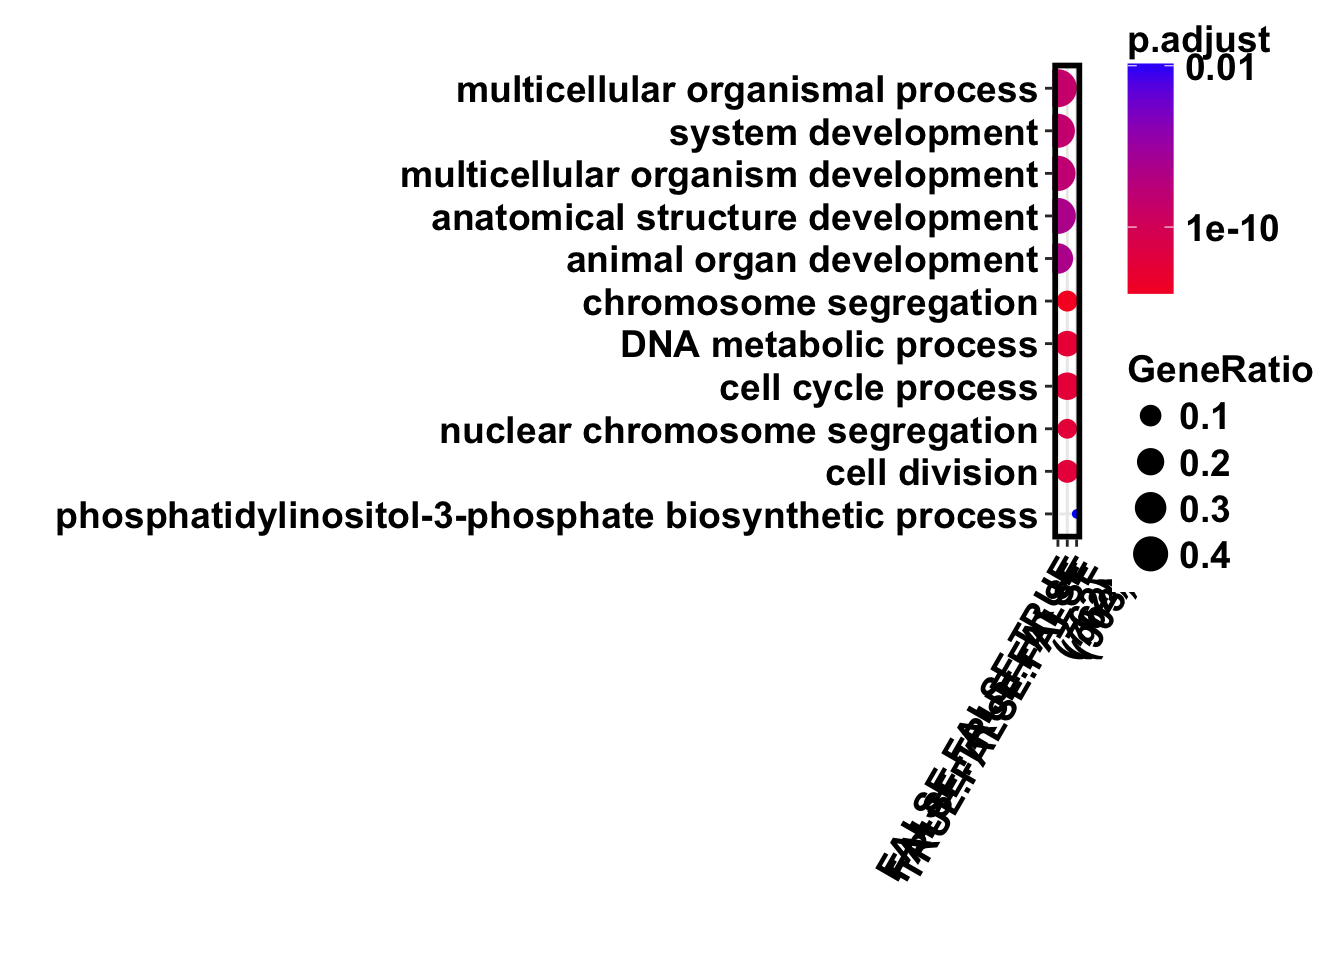
\includegraphics{figure/GO_motif_analysis.Rmd/unnamed-chunk-7-1} \end{center}


\end{document}
